\documentclass{oblivoir}
\usepackage{amsmath,amssymb,amsthm,kotex,mdframed,paralist,kswrapfig}

\newcounter{num}
\newcommand{\prob}
{\bigskip\noindent\refstepcounter{num}\textbf{문제 \arabic{num})}\par}

\newcommand{\ans}{{\raggedleft\textbf{답 : (\qquad\qquad\qquad\qquad\qquad\qquad)}
\par}\bigskip\bigskip}

\newcommand\ga{\text{(가)}}
\renewcommand\na{\text{(나)}}

%%%
\begin{document}
\Large

\title{승재 10 - 6학년 2학기 - 03}
\author{}
\date{\today}
\maketitle
%\tableofcontents

\newpage

%
\prob
다음 정사각형에서 색칠한 부분의 넓이를 구하세요.
\begin{figure}[h]
\centering
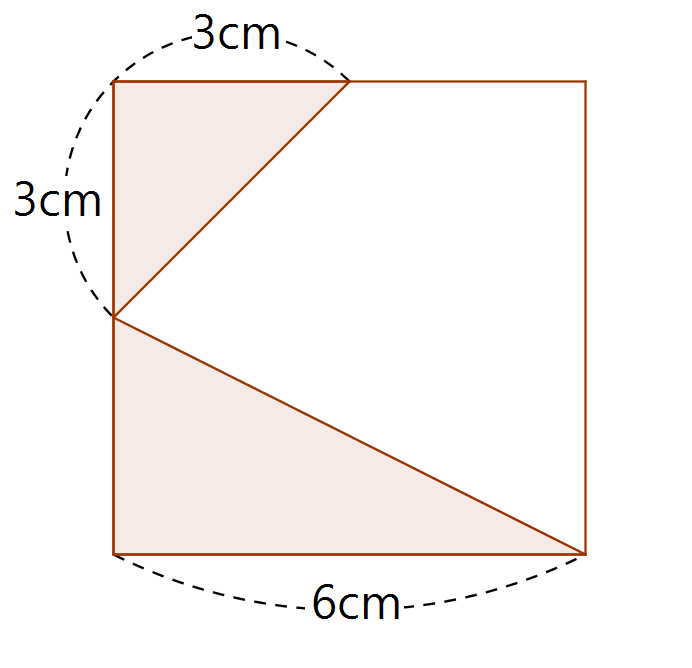
\includegraphics[width=0.5\textwidth]{01}
\end{figure}

\ans

\prob
다음 정사각형에서 색칠한 부분의 넓이를 구하세요.
\begin{figure}[h]
\centering
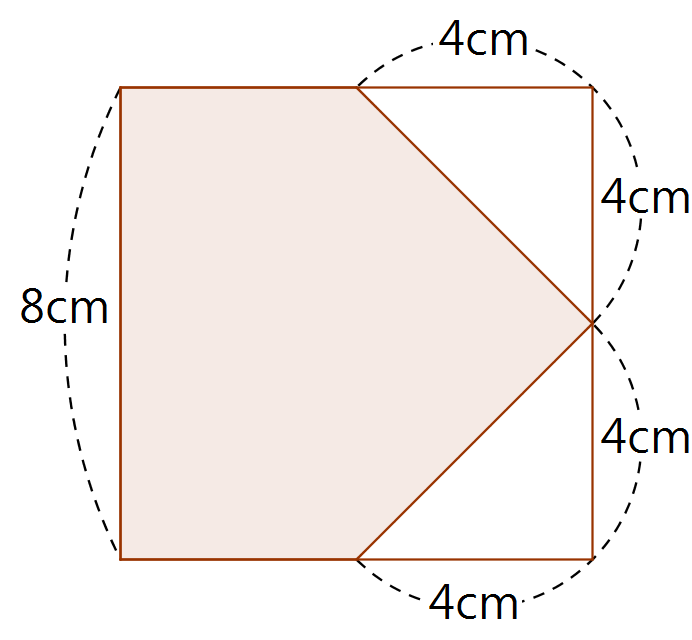
\includegraphics[width=0.5\textwidth]{02}
\end{figure}

\ans

\newpage
%
%\begin{figure}[h]
%\centering
%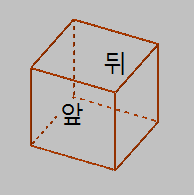
\includegraphics[width=0.5\textwidth]{a_cube}
%\end{figure}


\prob
한 모서리의 길이가 8cm이고 투명한 정육면체의 앞면과 뒷면에 각각 직사각형과 삼각형을 그린 후 색칠했습니다.
이 정육면체를 앞에서 볼 때, 색칠된 부분의 넓이를 구하시오.

\begin{figure}[h]
\centering
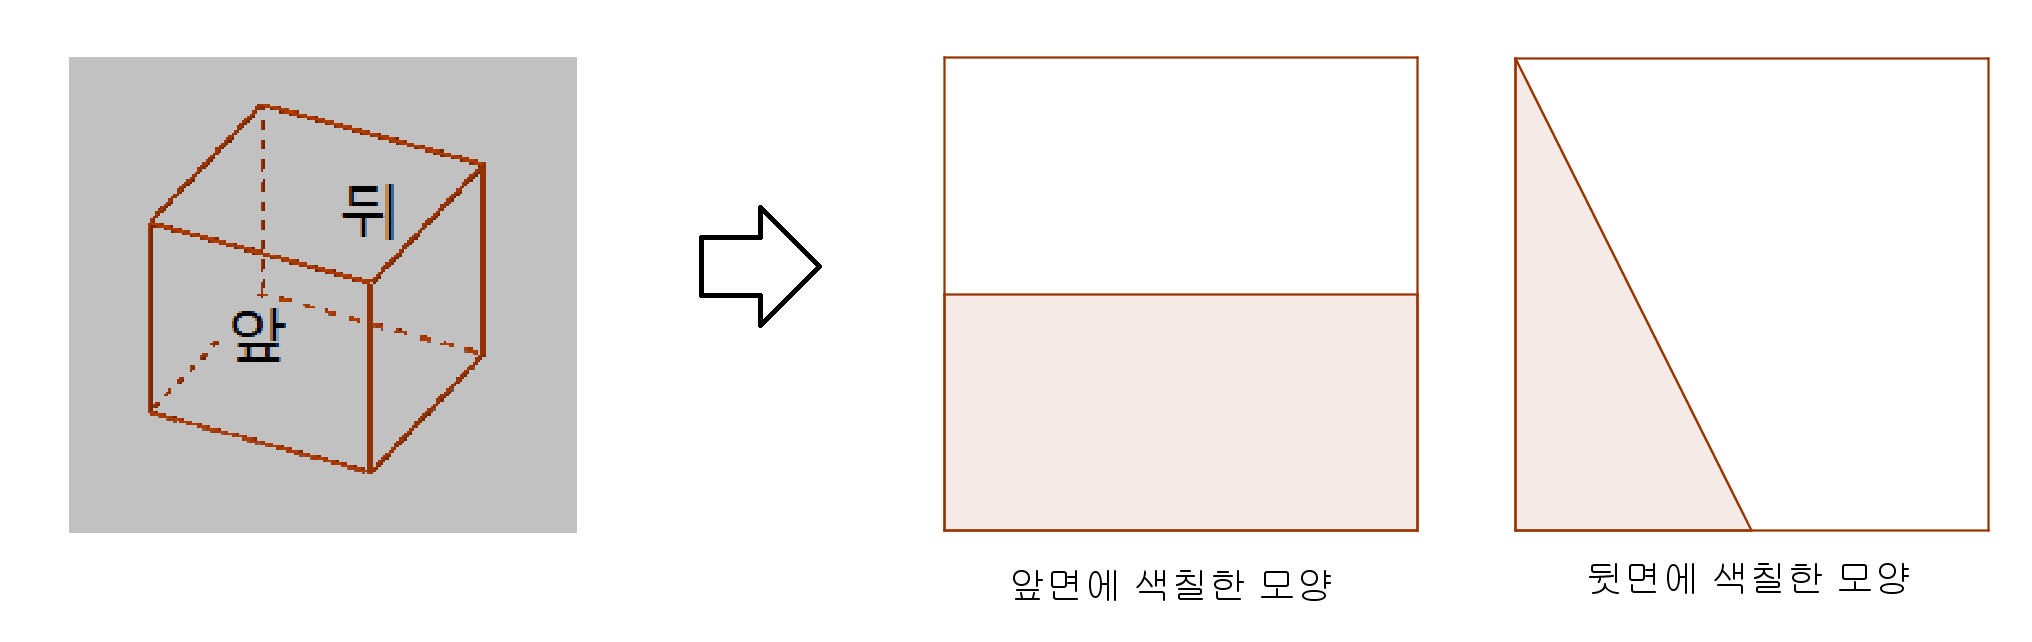
\includegraphics[width=\textwidth]{03}
\end{figure}

\ans

\prob
한 모서리의 길이가 6cm이고 투명한 정육면체의 앞면과 뒷면에 삼각형을 그린 후 색칠했습니다.
이 정육면체를 앞에서 볼 때, 색칠된 부분의 넓이를 구하시오.

\begin{figure}[h]
\centering
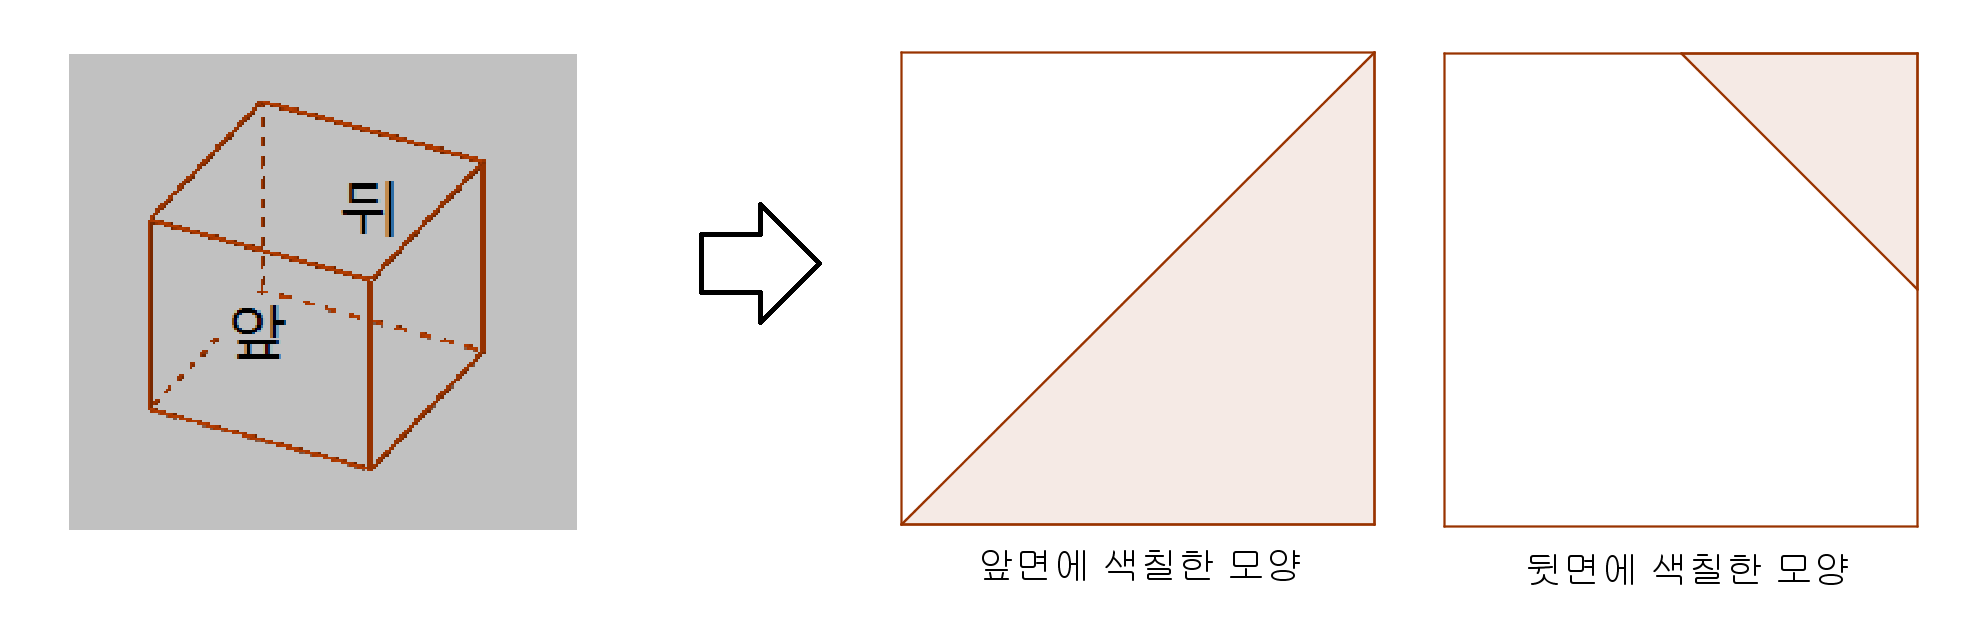
\includegraphics[width=\textwidth]{04}
\end{figure}

\ans

\newpage

\prob
비 (가) : (나)를 가장 간단한 자연수의 비로 나타내어 보시오.
\[
\ga\times1\frac45=\na\times\frac74
\]
\ans

\prob
비 (가) : (나)를 가장 간단한 자연수의 비로 나타내어 보시오.
\[
\ga\times2\frac32=\na\times1\frac14
\]
\ans

\prob
비 (가) : (나)를 가장 간단한 자연수의 비로 나타내어 보시오.
\[
\ga\times\frac74=\na\times\frac{27}2
\]
\ans

\prob
비 (가) : (나)를 가장 간단한 자연수의 비로 나타내어 보시오.
\[
\ga\times7\frac85=\na\times4\frac12
\]
\ans

\newpage

\prob
(가)의 0.45는 (나)의 \(\displaystyle\frac58\)과 같을 때 (가) : (나)를 가장 간단한 자연수의 비로 나타내어 보시오.
\begin{figure}[h]
\centering
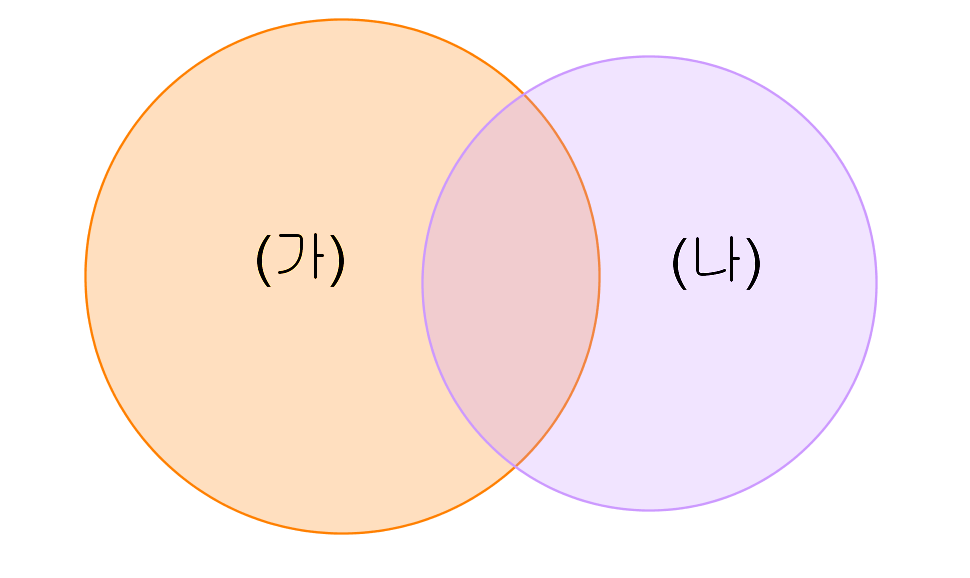
\includegraphics[width=0.5\textwidth]{09}
\end{figure}

\ans

\prob
(가)의 \(\displaystyle\frac5{16}\)는 (나)의 \(0.25\)과 같을 때 (가) : (나)를 가장 간단한 자연수의 비로 나타내어 보시오.
\begin{figure}[h]
\centering
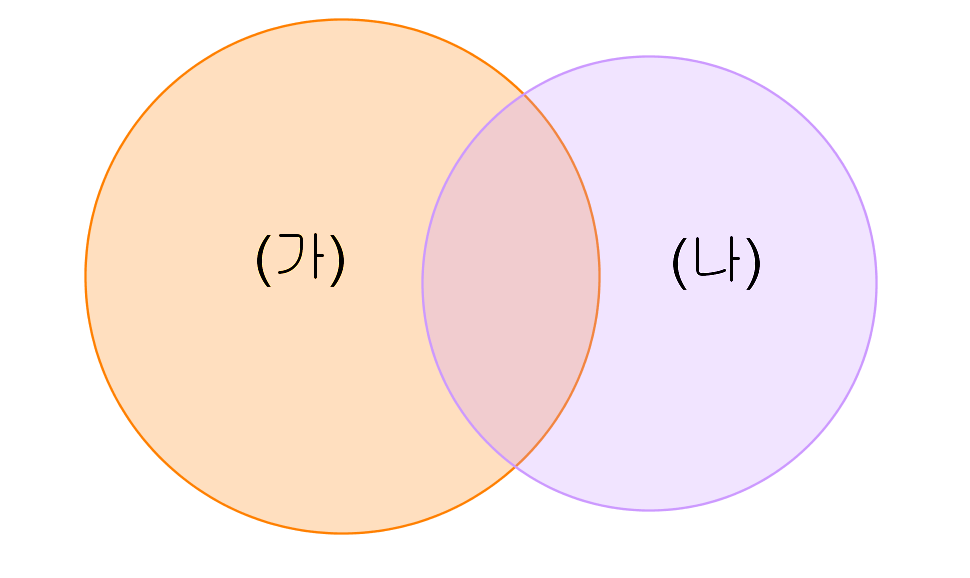
\includegraphics[width=0.5\textwidth]{09}
\end{figure}

\ans

\newpage

(1km=1000m이고, 1m=100cm이며 1cm=10mm입니다.
이것을 이용하여 다음 문제들을 풀어보세요.)

\prob
마라톤은 45.195km를 뛰는 운동경기입니다.
철수가 400m 둘레의 운동장을 35바퀴만큼 뛰었을 때, `철수가 달린 거리 : 마라톤 코스의 총 길이'를 가장 간단한 자연수의 비로 나타내세요.
\bigskip

{\raggedleft\textbf{
철수가 달린 거리 : 마라톤 코스의 총 길이 = (\qquad\quad:\qquad\quad)}
\par}\bigskip\bigskip

\prob
철수가 400m 둘레의 운동장을 몇 바퀴 돌아야 마라톤을 완주했다고 말할 수 있습니까?

\ans
\begin{figure}[h]
\centering
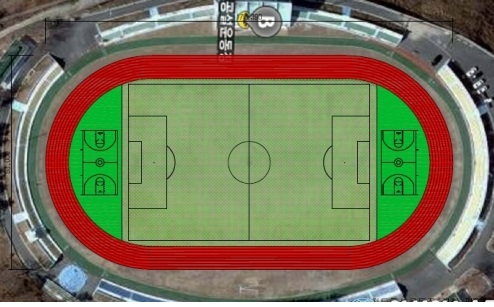
\includegraphics[width=0.7\textwidth]{track}
\end{figure}

\newpage

\prob
6.5mm길이의 일개미 400마리가 일렬로 늘어서 있습니다.
개미가 늘어선 길이와 몸길이가 4.5m인 악어의 길이의 비를 자연수의 비로 나타내세요.
(단, 개미 사이의 간격은 무시합니다.)

{\raggedleft\textbf{
개미가 늘어선 길이 : 악어의 길이 = (\qquad\quad:\qquad\quad)}
\par}\bigskip\bigskip


\ans
\begin{figure}[h]
\centering
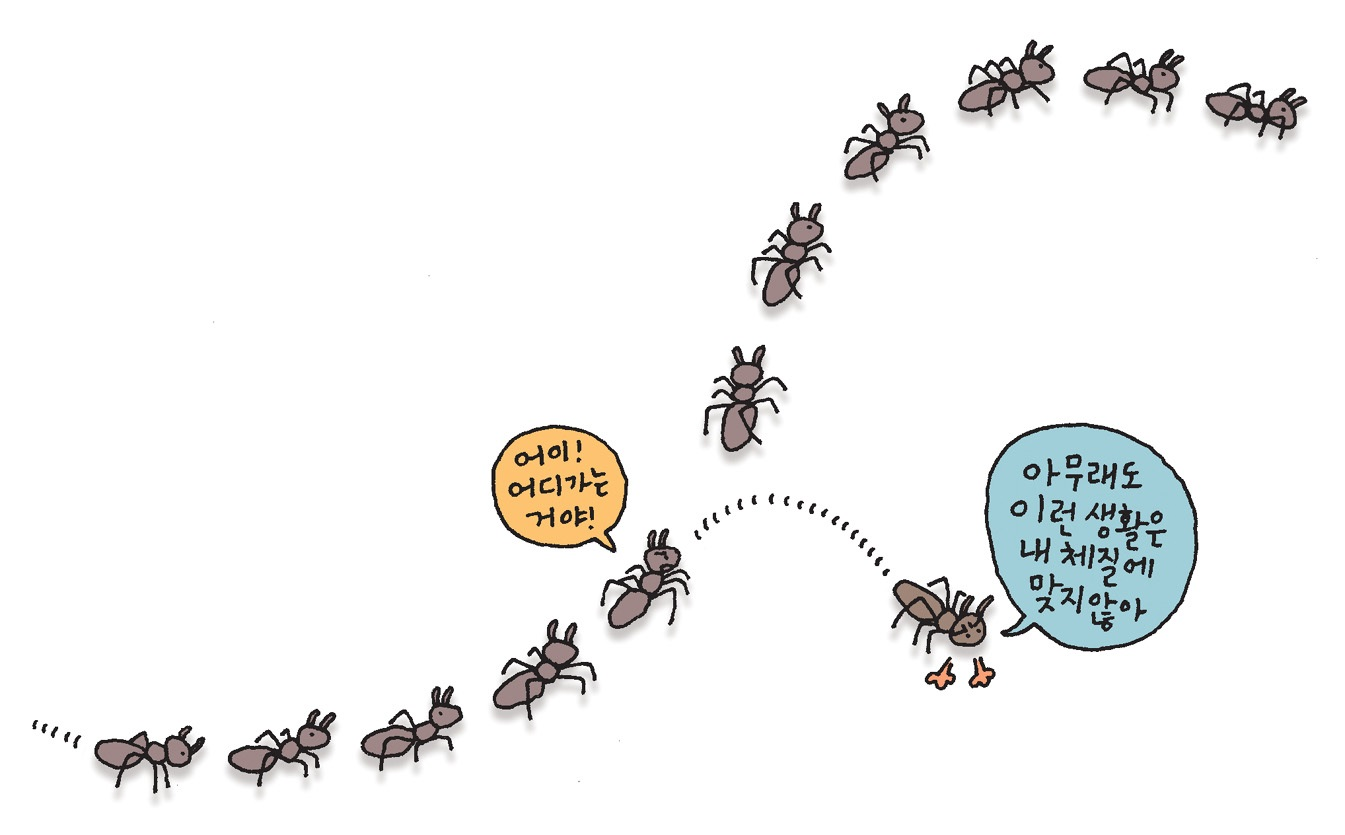
\includegraphics[width=0.7\textwidth]{ants}
\end{figure}

\newpage

\prob
고대 수학자인 탈레스는 피라미드 앞에 막대를 세워 놓고 피라미드의 그림자 길이와 막대의 그림자 길이를 잰 다음 비례식을 이용하여 거대한 피라미드의 높이를 재었습니다.
막대의 길이가 60cm, 막대의 그림자 길이가 130cm, 피라미드의 그림자의 길이가 5.2m일 때, 피라미드의 높이는 몇m인지 구하시오.
%{\center\small
%(막대 길이) : (막대의 그림자 길이) = (피라미드 높이) : (피라미드의 그림자 길이)
%}

\ans
\begin{figure}[h]
\centering
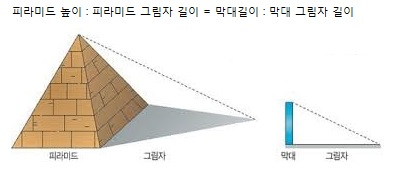
\includegraphics[width=0.8\textwidth]{pyramid}
\end{figure}


\end{document}